We consider a \emph{discrete memoryless quantum source} (DMQS) with generic density matrix $\rho \in \cS(\cH)$. In this model, the state of $n$ source outputs is the $n$-fold tensorial extension of the generic density matrix $\rho$, i.e.  
\begin{align*}
 \rho^{\otimes n} = \underbrace{\rho \otimes  \cdots \otimes \rho}_{n \ \text{times}}.
\end{align*}
In this lecture we consider the question to which extend the outputs of such a source can be compressed. We regard "degrees of freedom" i.e. "Hilbert space dimensions" as a costly resource and seek for source compression schemes, which map the statistics of the source outputs to a system with smaller number of dimensions such that it can be recovered in a sufficient way. \newline 
In case, that we aim to perfectly store $n$ outputs of the DMQS $\rho$, one can show, that a space of $(\rank\rho)^n$ dimensions is necessary. 
This amount can sometimes be decreased substantially, if we allow small imprecisions in recovery. A the general scheme of a source compression code for blocklength $n$ is depicted below. 
\begin{center}
    \vspace{2ex}
    \includegraphics[scale=.8]{pics/source_compression_scheme}
    \vspace{2ex}
   \end{center}
In order to show a coding theorem and a converse to quantify the asymptotics of the optimal compression rates, we need a sufficient performance measure to quantify the quality of recovery. We will use the \emph{entanglement fidelity} for this purpose. \newline 
In Section \ref{section:fidelity} we introduce (quantum) fidelity and entanglement fidelity. In Section 
\ref{section:source_compression}, we state and prove the source compression theorem for DMQS. Therein, the optimal compression rate will be 
determined by the von Neumann entropy of the generic density matrix. We discuss some properties of this function in Section \ref{section:von_neumann_entropy}.

\section{Fidelity, and Entanglement Fidelity} \label{section:fidelity} 
\begin{definition}[Quantum  fidelity \index{fidelity}] \label{def:fidelity}
 Let $A,B \in \cL(\cK)$, $A,B \geq 0$. The (quantum) fidelity of $A$ and $B$ is defined by
 \begin{align*} 
  F(A,B) := \|A^{\tfrac{1}{2}} B^{\tfrac{1}{2}} \|_1^2 = \left(\tr \left[ ( A^{\tfrac{1}{2}} B A^{\tfrac{1}{2}})^{\tfrac{1}{2}}\right]\right)^2. 
 \end{align*}
\end{definition}
%\begin{remark}
% There are two concurrent definitions of the quantum fidelity in the literature. Sometimes it is defined as the square-root of the function $F$ introduced in Def. %\ref{def:fidelity}.
%\end{remark}

\begin{lemma} \label{lemma:fidelity_properties}
 For $A,B \in \cL(\cK)$, $A, B \geq 0$, it holds
 \begin{enumerate}
  \item $F(A,B) \ = \ F(B,A)$, 
  \item $F(\lambda A, B) \ = \ \lambda F(A, B)$ for all $\lambda \geq 0$,
  \item $F( \ket{\psi}\bra{\psi}, B) \ = \ \braket{\psi, B \psi}$ for all $\psi \in \cK$, and 
  \item $0 \leq F(A,B) \leq 1$ for density matrices $A,B$.
  \end{enumerate}
\end{lemma}

The following theorem is a very important structural assertion for the quantum fidelity. It rephrases the fidelity as resulting from an optimization of the overlaps of purifications of the states. 
\begin{theorem}[Uhlmanns Theorem] \label{theorem:uhlmanns_thm} \index{theorem! Uhlmann's theorem}
Let $\rho, \sigma \in \cS(\cK)$. It holds 
\begin{align}
F(\rho, \sigma) \ = \ \max\left\{|\braket{\psi, \varphi}|^2: \ \psi \ \text{is purification of}\ \rho, \ \varphi \ \text{is purification of} \ \sigma \right\}.
\label{theorem:uhlmanns_thm_eq}
\end{align}
\end{theorem}
Before we give a proof of Uhlmanns theorem, we state and prove two supporting lemmas. The first one is a variational characterization of the trace norm. 
\begin{lemma} \label{lemma:tracenorm_variation}
 Let $A \in \cL(\cH)$. It holds
 \begin{align}
  \|A\|_1 := \max \left\{|\tr AU|: \ U \in \cL(\cH) \ \text{unitary} \right\}. \label{var_tracenorm_lemma_1}
 \end{align}
\end{lemma}
\begin{proof}
 Let 
  $
  A = U_0|A|
  $
 be a polar decomposition of $A$ (remember the definition $|A| = \sqrt{A^\ast A}$), and 
 \begin{align*}
  |A| = \sum_{i=1}^m a_i \ket{\varphi_i}\bra{\varphi_i}
 \end{align*}
 be a spectral decomposition of $|A|$. Let $U$ be any unitary on $\cH$ and define $V:= UU_0$ (which is also a unitary matrix!). We have
 \begin{align*}
  |\tr(AU)| 
  & = |\tr(|A|V)|  \\
%  & = |\sum_{i=1}^m a_i \tr(\ket{\varphi_i}\bra{\varphi_i}V)| \\
  & = |\sum_{i=1}^m a_i \braket{\varphi_i, V \varphi_i}| \\
  & \leq \sum_{i=1}^m a_i |\braket{\varphi_i, V \varphi_i}| \\
  & \leq \sum_{i=1}^m a_i \\
  & = \tr|A| \\
  &= \|A\|_1.
 \end{align*}
  The first inequality above is the triangle inequality. The second one follows from the fact, that $V$ is a unitary. The last equality is by definition of the trace norm. Therefore the right hand side is dominated by the left hand side in (\ref{var_tracenorm_lemma_1}). On the other hand, the reverse inequality also holds (\ref{var_tracenorm_lemma_1}) is achieved. Indeed, it holds
 \begin{align*}
  |\tr(AU_0^\ast)| = \tr(|A|) = \|A\|_1.
 \end{align*}
\end{proof} 
\begin{lemma} \label{lemma:entanglement_trick}
 Let $\{\varphi_i\}_{i=1}^d$ an orthonormal basis in $\cK$, $\dim \cK := d$. And let $\phi \in \cK \otimes \cK$ be defined by $
  \phi := \sum_{i =1}^d \varphi_i \otimes \varphi_i.
  $
 It holds
 \begin{align*}
  (A \otimes \bbmeins_{\cK}) \phi = (\bbmeins_\cK \otimes A^T) \phi 
 \end{align*}
 where $A^T$ is the transpose of $A$ with respect to $\{\varphi_i\}_{i=1}^d$ \footnote{Note that the transposed matrix depends on the chosen basis}.
\end{lemma}
 \begin{proof}
  Let 
$ 
   A = \sum_{i,k=1}^d a_{ij} \ket{\varphi_i}\bra{\varphi_j},
 $
  (written as a linear combination in the $\{\ket{\varphi_i}\bra{\varphi_j}\}_{i,j=1}^d$ basis.) Straightforward calculation then gives 
  \begin{align*}
   (A \otimes \bbmeins_\cK)\ket{\phi}
   & = \sum_{i=1}^d A \ket{\varphi_i} \otimes \ket{\varphi_i} \\
   & = \sum_{i,k,l =1}^d a_{kl} \ket{\varphi_k}\bra{\varphi_l}\ket{\varphi_i} \otimes \ket{\varphi_i} \\
   & = \sum_{k,i =1}^d a_{ki} \ket{\varphi_k} \otimes \ket{\varphi_i} \\
   & = \sum_{k =1}^d\left( \ket{\varphi_k} \otimes \sum_{i =1}^d a_{ki}\ket{\varphi_i} \right) \\
   & = \sum_{k =1}^d \ket{\varphi_k} \otimes \left(\sum_{l,i =1}^d a_{li}\ket{\varphi_i} \braket{\varphi_l,\varphi_k}\right) \\
   & = \sum_{k =1}^d \ket{\varphi_k} \otimes A^T \ket{\varphi_k} \\
   & = (\bbmeins_\cK \otimes A^T) \ket{\phi}
  \end{align*}
 \end{proof}
   \begin{proof}[Proof of Theorem \ref{theorem:uhlmanns_thm}]
  Let $\psi, \varphi$ be unit vectors in $\cK \otimes \cK$, and assume, that $\psi$ is state vector of a purification of $\rho$ and $\varphi$ is state vector of a purification of $\sigma$. Let 
  \begin{align*}
   \psi \ = \ \sum_{k=1}^d \sqrt{\mu_k} \psi_k \otimes \gamma_k, \hspace{.5cm} \text{and} \hspace{1cm}
   \varphi \ = \ \sum_{l=1}^d \sqrt{\vartheta_l} \varphi_l \otimes \tau_l 
  \end{align*}
   be Schmidt decompositions of $\psi$ resp. $\varphi$ (some Schmidt coefficients may vanish). Let $U_1, U_2, V \in \cL(\cK)$ be unitaries such that for each $k \in [d]$ the equalities
   \begin{align*}
    \varphi_k = V \psi_k, \hspace{.5cm} 
    \gamma_k  = U_1 \psi_k, \ \text{and} \hspace{.5cm}
    \tau_m = U_2 \varphi_k
   \end{align*}
   hold. Definition of the square root function, we have the eigenvalue equations 
   \begin{align}
    \sqrt{\mu_k} \psi_k = \rho^{\tfrac{1}{2}} \psi_k  \hspace{.5cm}
    \sqrt{\vartheta_k} \varphi_k = \sigma^{\tfrac{1}{2}} \varphi_k
   \end{align}
    It holds
   \begin{align}
    \psi 
    &\ = \ \sum_{k=1}^d \sqrt{\mu_k} \psi_k \otimes \gamma_k \nonumber \\
    &\ = \ (\rho^{\tfrac{1}{2}} \otimes \bbmeins_\cK)\sum_{k=1}^d \psi_k \otimes \gamma_k \nonumber \\
    &\ = \ (\rho^{\tfrac{1}{2}} \otimes \bbmeins_\cK)\sum_{k=1}^d \psi_k \otimes U_1\psi_k \nonumber \\
    &\ = \ (\rho^{\tfrac{1}{2}} \otimes U_1)\sum_{k=1}^d \psi_k \otimes \psi_k \nonumber \\
    &\ = \ (\rho^{\tfrac{1}{2}}U_1^T \otimes \bbmeins_\cK)\sum_{k=1}^d \psi_k \otimes \psi_k. \label{proof_uhlmanns_thm_1}
   \end{align}
    The last of the equalities above is by Lemma \ref{lemma:entanglement_trick}. By a very similar calculation as done above for $\psi$, also
    \begin{align*}
     \varphi \ = \ (\sigma^{\tfrac{1}{2}}U_2^T \otimes \bbmeins_\cK)\sum_{k=1}^d \varphi_k \otimes \varphi_k
    \end{align*}
    holds. We further calculate
    \begin{align}
     \varphi 
     &\ = \ (\sigma^{\tfrac{1}{2}}U_2^T \otimes \bbmeins_\cK)\sum_{k=1}^d V\psi_k \otimes V\psi_k \\
     &\ = \ (\sigma^{\tfrac{1}{2}}U_2^TVV^T \otimes \bbmeins_\cK)\sum_{k=1}^d \psi_k \otimes \psi_k, \label{proof_uhlmanns_thm_2}
    \end{align}
     where we once more used Lemma \ref{lemma:entanglement_trick} to obtain the last equality above. With (\ref{proof_uhlmanns_thm_1}) and (\ref{proof_uhlmanns_thm_2}), we calculate
     \begin{align*}
      \braket{\psi, \varphi} 
      & = \sum_{k,l=1}^d \braket{(\rho^{\tfrac{1}{2}}U_1^T \otimes \bbmeins_\cK)\psi_k \otimes \psi_k, (\sigma^{\tfrac{1}{2}}U_2^TVV^T \otimes \bbmeins_\cK) \psi_l \otimes \psi_l} \\
      & = \sum_{k,l=1}^d \braket{\psi_k \otimes \psi_k, (\rho^{\tfrac{1}{2}}U_1^T \otimes \bbmeins_\cK)^\ast (\sigma^{\tfrac{1}{2}}U_2^TVV^T \otimes \bbmeins_\cK) \psi_l \otimes \psi_l} \\
      & = \sum_{k,l=1}^d \braket{\psi_k \otimes \psi_k, (\overline{U}_1\rho^{\tfrac{1}{2}}\sigma^{\tfrac{1}{2}}U_2^TVV^T \otimes \bbmeins_\cK) \psi_l \otimes \psi_l} \\
      & = \sum_{k,l=1}^d \braket{\psi_k, \overline{U}_1\rho^{\tfrac{1}{2}}\sigma^{\tfrac{1}{2}}U_2^TVV^T \psi_l} \cdot \braket{\psi_k, \psi_l}\\
      & = \sum_{k=1}^d \braket{\psi_k, \overline{U}_1\rho^{\tfrac{1}{2}}\sigma^{\tfrac{1}{2}}U_2^TVV^T \psi_k} \\
      & = \tr(\overline{U}_1\rho^{\tfrac{1}{2}}\sigma^{\tfrac{1}{2}}U_2^TVV^T).
      \end{align*}
      The above chain of equations yields 
      \begin{align}
       |\braket{\psi, \varphi}| \ = \ |\tr(\rho^{\tfrac{1}{2}}\sigma^{\tfrac{1}{2}}U_2^TVV^T\overline{U}_1)| \label{eq_unitaries_uhlmann}
      \end{align}
      We note, that $U_2^TVV^T\overline{U}_1$ is a unitary matrix. Furthermore, $U_1, U_2, V$ depend on the choice of purifications of the state. In fact, each unitary on $\cK$ can be realized by $U_2^TVV^T\overline{U}_1$ by choosing corresponding purifications. If we choose purifications, such that right hand side of Eq. (\ref{eq_unitaries_uhlmann}) is maximal, we obtain using  
      Lemma \ref{lemma:tracenorm_variation} the claim of the Theorem. 
 \end{proof}

\begin{definition}[Entanglement fidelity \index{fidelity!entanglement fidelity}]
Let $\rho \in \cS(\cK)$, $\cN \in \cC(\cK,\cK)$.  The entanglement fidelity of $(\rho, \cN)$ is defined by
\begin{align}
 F_e(\rho, \cN) := F(\ket{\psi} \bra{\psi}, \id_{\cK} \otimes \cN(\ket{\psi}\bra{\psi}) = \braket{\psi, \id_{\cK} \otimes \cN (\ket{\psi}\bra{\psi}) \psi},
\end{align}
where $\psi$ is the state vector of a purification of $\rho$. 
\end{definition}
 The reader may ask, whether or not the entanglement fidelity is well-defined. This question is affirmatively answered by the statement of the following lemma. In fact, one consequence of the 
 representation in terms of Kraus operators given below is, that the entanglement fidelity does 
 not depend on the chosen purification of the argument.
\begin{lemma} \label{lemma:entanglement_fidelity_kraus_dec}
 Let $\cN \in \cC(\cK, \cK)$ and
 $
  \cN(x) = \sum_{k=1}^N A_k x A_k^\ast  \ (x \in \cL(\cK))
 $
 a Kraus decomposition of $\cN$. It holds for each $\rho \in \cS(\cK)$
 \begin{align}
  F_e(\rho,\cN) = \sum_{k=1}^N |\tr(A_k\rho)|^2 
 \end{align}
  \end{lemma}
 \begin{proof}
   Let $\psi$ be the state vector of any purification of $\rho$ with Schmidt decomposition
$
    \psi = \sum_{i=1}^d \sqrt{\lambda_i} \ \gamma_i \otimes \vartheta_i.
 $
   Define $\tilde{\vartheta}_i := \sqrt{\lambda_i} \vartheta_i$ for each $i \in [d]$.  It holds
   \begin{align}
    \psi = \sum_{i=1}^d \gamma_i \otimes \tilde{\vartheta}_i, \hspace{.3cm} \text{and} \hspace{.5cm} \rho = \sum_{i=1}^d \ket{\tilde{\vartheta}_i} \bra{\tilde{\vartheta}_i} 
   \end{align}
  We calculate 
  \begin{align}
   \braket{\psi, \id_{\cK} \otimes \cN(\ket{\psi}\bra{\psi}) \psi} \ 
   & = \ \sum_{i,j,l,m =1}^d \ \braket{\gamma_i \otimes \tilde{\vartheta}_i, 
    (\id_{\cK} \otimes \cN)(\ket{\gamma_j \otimes \tilde{\vartheta}_j}\bra{\gamma_l \otimes \tilde{\vartheta}_l}), \gamma_m \otimes \tilde{\vartheta}_m} \nonumber \\
   & = \sum_{i,l = 1}^d \ \braket{\tilde{\vartheta}_i, \cN(\ket{\tilde{\vartheta}_i}\bra{\tilde{\vartheta}_l}), \tilde{\vartheta_l}}. \label{lemma:entanglement_fidelity_kraus_dec_1}
  \end{align}
  For each $i,l \in [d]$, the summand on the r.h.s. of the equality in (\ref{lemma:entanglement_fidelity_kraus_dec_1}) can be further written as
  \begin{align}
   \braket{\tilde{\vartheta}_i, \cN(\ket{\tilde{\vartheta}_i}\bra{\tilde{\vartheta}_l}), \tilde{\vartheta_l}} \
     = \ \sum_{k=1}^N  \braket{\tilde{\vartheta}_i, A_k\ket{\tilde{\vartheta}_i}\bra{\tilde{\vartheta}_l}A_k^{\ast}, \tilde{\vartheta_l}} \nonumber 
%   & = \ \sum_{k=1}^N \braket{\tilde{\vartheta}_i, A_k \tilde{\vartheta}_i} \overline{\braket{\tilde{\vartheta}_l, A_k \tilde{\vartheta}_l}} \nonumber \\
    \ = \ \sum_{k=1}^N \tr \ket{\tilde{\vartheta}_i}\bra{\tilde{\vartheta}_i}A_k  \ \cdot \  \overline{\tr \ket{\tilde{\vartheta}_l}\bra{\tilde{\vartheta}_l}A_k}.  \label{lemma:entanglement_fidelity_kraus_dec_2}
  \end{align}
  Combination of (\ref{lemma:entanglement_fidelity_kraus_dec_1}) with (\ref{lemma:entanglement_fidelity_kraus_dec_2}) leads us to
  \begin{align*}
   \braket{\psi, \id_{\cK} \otimes \cN(\ket{\psi}\bra{\psi}) \psi} \ 
   & = \ \sum_{k=1}^N \sum_{i,l=1}^d \tr \ket{\tilde{\vartheta}_i}\bra{\tilde{\vartheta}_i}A_k  \ \cdot \  \overline{\tr \ket{\tilde{\vartheta}_l}\bra{\tilde{\vartheta}_l}A_k} \\
   & = \ \sum_{k=1}^N \tr \sum_{i=1}^d \ket{\tilde{\vartheta}_i}\bra{\tilde{\vartheta}_i}A_k  \ \cdot \  \overline{\tr \sum_{l=1}^d \ket{\tilde{\vartheta}_l}\bra{\tilde{\vartheta}_l}A_k} \\
   & = \ \sum_{k=1}^N |\tr A_k \rho |^2.
  \end{align*}
 \end{proof}
\section{Quantum Source Compression} \label{section:source_compression}
In this section, we will determine the optimal rate for compression of a DMQS. We define  
\begin{definition}
 An \emph{$(n,k)$-code for source compression} of the DMQS $\rho \in \cS(\cH)$ is a pair $(\cE,\cD)$, where $\cE \in \cC(\cH^{\otimes n}, \cK)$, $\cD \in \cC(\cK, \cH^{\otimes n})$ are c.p.t.p. maps, and $k = \dim \cK$. 
 We define for each $n \in \bbmN, \epsilon \geq 0$
 \begin{align*}
  K(\rho, n, \epsilon) \ := \ \min\left\{k: \ \exists(n,k) \text{-code} \ (\cE, \cD) \ \text{with} \ F_e(\rho^{\otimes n}, \cD \circ \cE) \geq 1 - \epsilon \right\}
 \end{align*}
\end{definition}
The following assertion is known as the source compression theorem for discrete memoryless quantum sources.

\begin{theorem}[DMQS Source compression theorem] \label{thm:q_source_compression}
 Let $\rho \in \cS(\cH)$. It holds for all $\epsilon \in (0,1)$ 
 \begin{align*}
  \underset{n \rightarrow \infty}{\lim} \frac{1}{n} \log K(\rho, n, \epsilon) \ = \ S(\rho).
 \end{align*}
 \end{theorem}
 The above theorem provides the von Neumann entropy $S$ with an operational meaning. $S(\rho)$ is 
 the minimal compression rate for asymptotically perfect compression of the DMQS $\rho$. 
 Before we prove the theorem, we first recall some statements, we already have proven in Lemma \ref{lemma:steins_lemma_projection}. 
\begin{lemma}
 Let $\rho \in \cS(\cH)$ be a quantum state, $\delta > 0$. There exists a sequence $\{p_n\}_{n=1}^\infty$ of orthogonal projections such that for each $n \in \bbmN$
 \begin{enumerate} \label{lemma:source_compression_lemma}
  \item $[p_n, \rho^{\otimes n}] = 0$, \label{lemma:source_compression_lemma_1}
  \item $2^{-n(S(\rho) + \delta))} p_n \ \leq \ p_n \rho^{\otimes n} p_n \ \leq \ 2^{-n(S(\rho) - \delta))} p_n$, 
  \item $\tr p_n \leq 2^{n(S(\rho) + \delta))}$ , and moreover \label{lemma:source_compression_lemma_4}
  \item $\underset{n \rightarrow \infty}{\lim} \ \tr p_n  \rho^{\otimes n} \ = \ 1$ \label{lemma:source_compression_lemma_5}
  \end{enumerate}
\begin{proof}
 The claims follow from Lemma \ref{lemma:steins_lemma_projection} with $\tau_1 = \tau_2 = 1$. The bound on the rank of $p_n$ in \ref{lemma:source_compression_lemma}.\ref{lemma:source_compression_lemma_4} 
 follows by 
 \begin{align*}
  \tr p_n \leq 2^{n(S(\rho) + \delta)} \cdot \tr p_n \rho^{\otimes n} \ \leq \ 2^{n(S(\rho) + \delta)}.
  \end{align*}

\end{proof}
\end{lemma}
We will first show the achievability part of Theorem \ref{thm:q_source_compression}. 
\begin{proposition} \label{source_compression_achiev} 
 Let $\rho \in \cS(\cH)$. It holds
 \begin{align}
  \underset{n  \rightarrow \infty}{\limsup} \ \frac{1}{n} \log K(\rho, n, \epsilon) \ \leq S(\rho) %\label{source_compression_achiev_1}
 \end{align} 
 for all $\epsilon > 0$. 
\end{proposition}
\begin{proof}
 Let $\epsilon \in (0,1)$, $\delta > 0$ be arbitrary but fixed numbers, and $p_n$ for each $n \in \bbmN$ the projection from 
 Lemma \ref{lemma:source_compression_lemma}. We show, that the inequality
 \begin{align}
  K(\rho, n, \epsilon)  \ \leq \ 2^{n(S(\rho) + \delta)} \label{source_compression_achiev_1}
 \end{align}
 holds for each large enough blocklength $n$ (for all $n > n_0 := \min\left\{n \in \bbmN: \ \tr(p_n \rho^{\otimes n}) > \sqrt{1 -\epsilon} \right\}$).
 We define the shorthands
$
  p_n^{\perp} := \bbmeins_{\cH^{\otimes n}} - p_n$, and$\cK_n := \supp(p_n).
 $
 Fix a blocklength $n > n_0$. Define encoding and decoding channels $\cE_n \in \cC(\cH^{\otimes n}, \cK)$, and $\cD_n \in \cC(\cK_n, \cH^{\otimes n})$ by 
 \begin{align*}
  \cE_n(A) &:= p_n A p_n^\ast + \tr(p_n^{\perp}) \frac{p_n}{\tr(p_n)}   &(A \in \cL(\cH^{\otimes n})), \ \text{and} \\
  \cD_n(B) &:= VBV^\ast  & (B \in \cL(\cK_n)),
 \end{align*}
  where $V: \cK_n \rightarrow \cH^{\otimes n}$ is the injection of the subspace $\cK_n$ into $\cH^{\otimes n}$. Let 
$
   \cE_n(\cdot) \ := \ \sum_{k=1}^N \ E_k (\cdot) E_k^{\ast} 
 $
  be a Kraus decomposition of  $\cE_n$ with $E_1 := p_n$ (check, that this is in fact possible). Using the corresponding Kraus decomposition 
  \begin{align*}
   \cD_n \circ \cE_n(A) := \sum_{k=1}^N VE_k A (VE_k)^{\ast}  &&(A \in \cL(\cH^{\otimes k})) 
  \end{align*} 
   of the composition of encoding and decoding, $\cD_n \circ \cE_n$, we calculate
  \begin{align}
   F_e(\rho^{\otimes n}, \cD_n \circ \cE_n) 
   & = \sum_{k=1}^N |\tr(VE_k \rho^{\otimes n})|^2  \label{source_compression_achiev_3} \\
   & \geq |\tr(VE_1 \rho^{\otimes n})|^2 \nonumber  \nonumber \\
   & =  |\tr(p_{n} \rho^{\otimes n})|^2  \nonumber  \nonumber \\
   &\geq 1 - \epsilon.  \label{source_compression_achiev_6}
  \end{align}
  By the inequality in (\ref{source_compression_achiev_6}), we have
  \begin{align}
    K(\rho,n, \epsilon) \ \leq \  \dim \cK_n \ \leq \  \tr(p_n) \ \leq \ 2^{n(S(\rho) + \delta)}.  \label{source_compression_achiev_7}
   \end{align}
   The rightmost inequality in (\ref{source_compression_achiev_7}) is from Lemma \ref{lemma:source_compression_lemma}.\ref{lemma:source_compression_lemma_4}. 
   We have shown the inequality in Eq. (\ref{source_compression_achiev_1}), which directly implies 
   \begin{align*}
    \underset{n \rightarrow \infty}{\limsup} \frac{1}{n} \log K(\rho, n, \epsilon) \leq S(\rho) + \delta.
   \end{align*}
   Since $\delta$ was an arbitrary positive number, we are done. 
\end{proof}

\begin{proposition}
 Let $\rho \in \cS(\cH)$. It holds  for all $\epsilon \in (0,1)$
 \begin{align*}
  \underset{n \rightarrow \infty}{\liminf}\frac{1}{n} \log K(\rho, n, \epsilon) \ \geq \ S(\rho).
 \end{align*}
\end{proposition}

\begin{proof}
 Fix $\epsilon \in (0,1)$, and abbreviate $K_n := K(\rho, n, \epsilon)$ $(n \in \bbmN)$. Let $(\cE_n,\cD_n)$ be 
 an $(n,K_n)$ source compression code for $\rho$ which fulfills
 \begin{align}
  F_e(\rho^{\otimes n}, \cD_n \circ \cE_n) \geq 1 - \epsilon.
 \end{align}
 Let 
 \begin{align*}
  \cE_n(A) &= \sum_{k=1}^N E_k A E_k^\ast &(A \in \cL(\cH^{\otimes n})), \\ 
  \cD_n(B) &= \sum_{l=1}^M D_l B D_l^\ast &(B \in \cL(\cK_n)) 
 \end{align*}
 be any Kraus decompositions of $\cE_n$, $\cD_n$. We represent the entanglement fidelity of the source compression protocol by means of its Kraus decompositions, we have,
 using Lemma \ref{lemma:entanglement_fidelity_kraus_dec},
 \begin{align} 
  F_e(\rho^{\otimes n}, \cD_n \circ \cE_n) = \sum_{k=1}^N \sum_{l=1}^M |\tr(D_lE_k\rho^{\otimes n}) |^2.
 \end{align}
 We define the shorthands $\sigma := \rho^{\otimes n}$, and 
$
  \Delta_{kl} := |\tr(D_l E_k \sigma)|^2
 $
 for each $l \in [N], \ l \in [M]$, and denote by $\hat{q}_l$ to be the projector onto the range of $D_l$, in particular we have $\hat{q}_l D_l x = D_l x $ for each $x \in \cK_n$. 
 We estimate
 \begin{align*}
  \Delta_{kl} 
  &= | \tr(\sigma^{\tfrac{1}{2}} D_l E_k \sigma^{\tfrac{1}{2}}) |^2 \\
  &= | \tr(\sigma^{\tfrac{1}{2}} \hat{q}_lD_l E_k \sigma^{\tfrac{1}{2}}) |^2 \\
  &= | \braket{\hat{q}_l \sigma^{\tfrac{1}{2}}, D_l E_k \sigma^{\tfrac{1}{2}}}_{HS} |^2 \\
  &\leq \|\hat{q}_l \sigma^{\tfrac{1}{2}} \|_2^2 \cdot \|D_l E_k \sigma^{\tfrac{1}{2}}\|_2^2 \\
  & = \tr(\hat{q}_l\sigma) \cdot \tr(E_k^\ast D_l^\ast D_l E_k \sigma). 
 \end{align*}
 The inequality above is the Cauchy-Schartz inequality. 
 Note, that with $p_n$ (the projector from Lemma \ref{lemma:source_compression_lemma})
 \begin{align*}
  \tr(\hat{q}_l q) \ \leq \ \tr(\hat{q_l}) \ =  \ \dim \textrm{range} D_l \ \leq \ \dim \cK_n \ = \ K_n
 \end{align*}
 holds. Consequently
 \begin{align*}
  \tr(\hat{q}_l p_n \rho^{\otimes n} p_n) \
   \leq  \ 2^{-n(S(\rho)-  \delta)} \tr(\hat{q}_l p_n) \ 
   \leq \ 2^{-n(S(\rho)-  \delta)} K_n.
 \end{align*}
  We the shortcut $c_{kl} := \tr(E_k^\ast D_l^\ast D_l E_l \rho^{\otimes n})$ for each $k \in [N], l \in [M]$.
  \begin{align}
   1 - \epsilon 
   & \leq \sum_{k=1}^N \sum_{l=1}^M \ \tr(\hat{q}_l \rho^{\otimes n}) c_{kl}  \nonumber \\
   & \leq \sum_{k=1}^N \sum_{l=1}^M \ \tr(\hat{q}_l (p_n + p_n^\perp) ) \rho^{\otimes n} (p_n + p_n^\perp) ) c_{kl} \nonumber \\
   & = \sum_{k=1}^N \sum_{l=1}^M \ \left(\tr(\hat{q}_l p_n \rho^{\otimes n} p_n) + \tr(\hat{q}_l p_n^\perp
	  \rho^{\otimes n}p_n^{\perp})  \right) c_{kl} \nonumber \\
   & \leq \sum_{k=1}^N \sum_{l=1}^M \left(2^{-n(S(\rho)- \delta)} K_n + 
   \tr p_n^\perp\rho^{\otimes n}\right)  c_{kl} \nonumber  \\
   &= 2^{-n(S(\rho)- \delta)} K_n + \tr p_n^\perp\rho^{\otimes n} \label{source_comp_conv_x}
  \end{align}
  The last equation above is by the fact, that by definition $c_{kl} \geq 0$ and by properties of the Kraus decomposition $\sum_{k,l} c_{kl} = 1$. 
  Rearranging the inequality in (\ref{source_comp_conv_x}), we obtain
   \begin{align*}
   K(\rho,n, \epsilon) \ \geq (1 - \epsilon -  \tr p_n^{\perp}\rho^{\otimes n}) \cdot 2^{n(S(\rho)- \delta)}.
  \end{align*}
  We conclude 
  \begin{align*}
   \liminf_{n \rightarrow \infty} \ \tfrac{1}{n} \log K(\rho,n, \epsilon) \ \geq S(\rho) - \delta. 
  \end{align*}
  Since $\delta > 0$ was arbitrary, we are done.
  \end{proof}
  We collect the obtained statements to prove the source compression theorem. 
  \begin{proof}[Proof of Theorem \ref{thm:q_source_compression}]
   It holds for each $\epsilon \in (0,1)$
   \begin{align*}
    \liminf_{n \rightarrow \infty} \tfrac{1}{n} \log K(\rho, n, \epsilon) 
    \ \geq \ S(\rho) \ \geq  \ 
    \limsup_{n \rightarrow \infty} \tfrac{1}{n} \log K(\rho, n, \epsilon).
   \end{align*}
  \end{proof}

\section{Supplement: Matrix Functions and some properties of the von Neumann entropy}\label{section:von_neumann_entropy}
We have seen, that the von Neummann entropy $S(\rho)$ of a density matrix $\rho$ has an interpretation as the optimal 
asymptotical rate for compression of the memoryless quantum source generated by $\rho$. Here we state and prove some 
properties of this function.  \newline 
First we show, that $S$ is a concave function on $\cS(\cH)$, i.e. the following statement. 
\begin{proposition} \label{prop:von_neumann_concavity} \index{entropy!von Neumann!concavity}
 Let $\rho_1, \rho_2 \in \cS(\cH)$, and $\lambda \in (0,1)$. It holds
 \begin{align}
  S(\lambda \rho_1 + (1-\lambda) \rho_2)\ \geq \ \lambda S(\rho_1) + (1-\lambda) S(\rho_2).
 \end{align}
\end{proposition}

\begin{proposition}[Peierl's Inequality \index{Peierl's inequality}]
 Let $f: I \rightarrow \bbmR$ be convex, and $\{v_1,\dots, v_n\} \subset \bbmC^n$ be an orthonormal basis. It 
 holds 
 \begin{align}
  \sum_{j=1}^n f(\braket{v_j, A v_j})  \ \leq \ \tr f(A)    
 \end{align}
 for each $A \in \cA_n(I) := \{A \in \bbmM_{n}: \ \spec(A) \subset I \}$. 
\end{proposition}
\begin{proof}
 Let 
 \begin{align}
  A = \sum_{j=1}^m \ a_j P_j
 \end{align}
 be spectral decomposition of $A$ with $a_1,\dots a_m \in I$ eigenvalues and $P_j$ being the projection onto the eigenspace
 corresponding to $a_j$ for each $j \in [m]$. By spectral calculus, $f(A)$ has spectral
 decomposition
 \begin{align}
  A = \sum_{j=1}^m \ f(a_j) P_j.
 \end{align}
 Let $v \in \bbmC^n$ be any unit vector. It holds
 \begin{align}
  \braket{v, f(A) v}
  &= \sum_{j=1}^m f(a_j) \braket{v, P_j v} \\
  &\geq f(\sum_{i=1}^m a_j \braket{v, P_j v}) \\
  &= f(\braket{v,Av}). 
 \end{align}
 The inequality above follows from convexity of $f$ together with the fact, that the term on the left-hand side is 
 actually a convex combination of function values. The inequality then is by Jensen's inequality. We can apply the 
 above inequality on all of the vectors $v_1,\dots,v_n$ and obtain 
 \begin{align}
  \tr f(A) = \sum_{i=1}^m \braket{v_i, f(A) v_i} \geq \sum_{i=1}^m f(\braket{v_i,A v_i}). 
 \end{align}
 \end{proof}

 \begin{proposition}\label{prop:convex_trace_function}
  If $f: I \rightarrow \bbmR$ is convex, then the corresponding trace functional $\tr f: \cA_n(I) \rightarrow \cL(\cH)^h$ 
  is convex. 
 \end{proposition}
 \begin{proof}
  Fix $\lambda \in (0,1)$, and $A, B \in \cA_n(I)$, and let $\{v_1,\dots, v_i\}$ be an orthonormal basis of eigenvectors to 
  \begin{align}
   \lambda A + (1 - \lambda) B
  \end{align}
  (denote the eigenvalue corresponding to $v_i$ by $\mu_i$.) Then, it holds
  \begin{align}
   \tr f(\lambda A + (1 - \lambda) B) \ 
   & = \ \sum_{j=1}^n f(\mu_j) \\
   & = \ \sum_{j=1}^n f(\braket{v_j, (\lambda A + (1 - \lambda) B ) v_j}) \\
   & = \ \sum_{j=1}^n f(\lambda \braket{v_j, \lambda A v_j}  + (1 - \lambda) \braket{v_j, B  v_j}) \\
   & \leq \ \lambda \sum_{j=1}^n f(\braket{v_j, A v_j})  +  (1 - \lambda)\sum_{j=1}^n f(\braket{v_j, B  v_j}) \\
   & \leq  \lambda \tr f(A) + (1 - \lambda)  \tr f(B).
  \end{align}
  The first inequality above is by convexity of $f$ (as a scalar function), the second is by Peierl's inequality 
  applied. 
  \end{proof}
  
  \begin{proof}[Proof of Proposition \ref{prop:von_neumann_concavity}]
   Proof is by application of Proposition \ref{prop:convex_trace_function}. Note, that with $f: [0,1] \rightarrow \bbmR$
   \begin{align}
    f(x) := \begin{cases}
             x \cdot \log x & \text{if} x \in (0,1) \\
             0              & \text{if} x = 0,
            \end{cases}
   \end{align}
   it holds
   \begin{align}
    S(\rho) =  - \tr f(\rho). \label{function_f_defined}
   \end{align}
   Since $f$ is convex on $[0,1]$, Proposition \ref{prop:convex_trace_function} tells us, that $-\tr f$ (and equivalently
   $S$) is concave.
  \end{proof}

  \begin{proposition}[Monotonicity of $S$ under pinching channels]\label{prop:von_neumann_pinching_mon}
  	Let $P_1,\dots,P_K \subset \cL(\cK)$ be mutually orthogonal projections (i.e. $P_k^\ast = P_k, P_kP_k = P_k$, and $P_kP_{k'} = 0, k' \neq k$. It holds
  	\begin{align}
  	S(\sum_{k=1}^K P_k \rho P_k) \ \geq \ S(\rho)
  	\end{align}
  	for all $\rho \in \cS(\cK)$.
  \end{proposition}
  
  \begin{proposition}[Almost-convexity of the von Neumann entropy] \label{prop:von_neumann_almost_convexity}
   Let $\{\rho_x\}_{x \in \cX} \subset \cS(\cK)$ be a finite family of density matrices, and $q \in \cP(\cX)$ a probability distribution. Define 
   \begin{align}
    \overline{\rho} := \sum_{x \in \cX} q(x) \rho_x. 
   \end{align}
   It holds
   \begin{enumerate}
    \item $S(\overline{\rho}) \leq \sum_{x \in \cX} q(x) S(\rho_x) + H(q)$. \label{prop:von_neumann_almost_convexity_1}
    \item Equality in \ref{prop:von_neumann_almost_convexity_1}. holds if and only if $\supp \rho_x \perp \supp \rho_{x'}$ for all $x \neq x'$.
   \end{enumerate}
  \end{proposition}
  \begin{proof}
  	We first prove the assertion in case of mixture of pure states. Let $\Psi_1, \dots, \Psi_M \in \cS(\cH)$ be pure states and $\mu \in \cP([M])$. We show
  	 \begin{align}
		S\left(\sum_{i=1}^M \mu(i) \ \Psi_i\right) \ \leq  H(\mu).
	 \end{align}
	Define, with an additional Hilbert space $\cH' \simeq \bbmC^M$, and an orthonormal basis $\{v_i\}_{i=1}^M$
	\begin{align}
		\psi := \sum_{i=1}^M \sqrt{\mu(i)} \ \psi_i \otimes v_i
	\end{align}
	Notice, that $\tr_{\cH'} \ket{\psi}\bra{\psi} = \sum_{i=1}^M \mu(i) \Psi_i := \overline{\sigma}$. With $\Psi := \ket{\psi}\bra{\psi}$, it also holds
	\begin{align}
	 S(\tr_\cH \Psi) \ = \ S(\tr_{\cH'}\Psi) = S(\overline{\sigma}).
	\end{align}
	Moreover, we have 
	\begin{align}
		\tr_{\cH} \Psi \ 
		= \ \sum_{i,j =1}^M \sqrt{\mu(i)\mu(j)} \braket{\psi_i, \psi_j} \ \ket{v_i}\bra{v_j}.
	\end{align}
	If we now apply the pinching channel $\cP(\cdot) := \sum_{k=1}^M \ket{v_k}\bra{v_k}(\cdot)\ket{v_k}\bra{v_k}$ on $\cH'$, we obtain
	\begin{align}
		 \cP(\tr_\cH \Psi) \ = \ \sum_{i=1}^M \mu(i) \ket{v_i}\bra{v_i}
	\end{align}
	which yields
	\begin{align}
		S(\cP(\tr_\cH \Psi)) \ = \ H(\mu).
	\end{align}
	Putting everything together, we have
	\begin{align}
	 S(\overline{\sigma}) \ 
      \leq \ S(\cP(\tr_\cH(\Psi)) \
	 = \ H(\mu).  
	\end{align}
	Note that the inequality above is by Proposition \ref{prop:von_neumann_pinching_mon}.
	The general mixed-state case now easily follows. Let for each $i \in [N]$
	\begin{align}
		\rho_{i} \ = \ \sum_{i=1}^{M_i} \mu_i(j) \ket{v_j^{(i)}}\bra{v_j^{(i)}}
	\end{align} 
	be a spectral decomposition of $\rho_{i}$. We then have
	\begin{align}
	 S\left(\sum_{i=1}^N \lambda(i) \rho_i\right) \ 
	 &= \ S\left(\sum_{i=1}^N \sum_{j=1}^{M_i} \lambda(i) \mu_i(j) \ket{v_j^{(i)}} \bra{v_j^{(i)}}\right) \\
	 &\leq \ - \sum_{i=1}^N \sum_{j=1}^{M_i} \lambda(i) \mu_i(j) \log \lambda(i) \mu_i(j) \label{prop_von_neumann_almost_convexity_fin_ineq} \\
	 & = H(\lambda) - \sum_{i=1}^N \lambda(i) S(\rho_i).
	\end{align}
	The inequality above is by applying the pure-state case. Rearrangement of the above inequalty proves the claim. Inspecting the inequality in (\ref{prop_von_neumann_almost_convexity_fin_ineq}) we also verify the second claim of the proposition. Therein equality holds, if all projections appearing in the sum are mutually orthogonal. 
  \end{proof}
  
  
  
  
  \begin{lemma} \label{entropy!von Neumann!Invariance under isometries}
  Let $v: \cH \rightarrow \cK$ an isometric linear map (i.e. $vv^\ast = \bbmeins_{\cH}$, and $v^\ast v$ is an orthogonal projection in $\cK$. Then 
  \begin{align}
     S(v\rho v^\ast) \ = \ S(\rho)
  \end{align}
  does hold for all $\rho \in \cS(\cH)$. In particular $S$ is invariant under unitaries.
  \end{lemma}
  \begin{proof}
  	Is clear. Isometries do not change the spectrum of a matrix including multiplicities. 
  \end{proof}
  \begin{lemma} \label{lemma:von_neumann_entropy_bounds}
  Let $\rho \in \cS(\cH)$. It holds
  \begin{align}
  0 \leq S(\rho) \leq \log \dim \cH.
  \end{align}
  \end{lemma}
  \begin{proof}
  	The bounds on $S(\rho)$ directly carry over from the Shannon entropy via spectral decomposition. We give a proof for the right hand inequality for convenience. Let $\{\lambda(x)\}_{x=1}^{d}$ the 
  	probability distribution arising from the spectrum of $\rho$ (counting multiplicities). Let $f$ 
  	be the function defined in (\ref{function_f_defined}). It holds
  	\begin{align*}
  	 S(\rho) \ = \ H(\lambda) \ = \ - \sum_{x=1}^d f(x) \ = - d \cdot \sum_{x=1}^d \frac{1}{d} f(\lambda(x)) \ \leq \ - d \cdot f\left(\sum_{x=1}^d \frac{\lambda(x)}{d}\right) \ = \ - d \cdot f\left(\frac{1}{d}\right) = \log d. 
  	\end{align*} 
  	The inequality above is by concavity of $f$.
  \end{proof}
  \begin{lemma} \label{lemma:von_neumann_subadditivity} \index{entropy!von Neumann!subadditivity}
   Let $\rho \in \cS(\cH \otimes \cK), \sigma_1 := \tr_\cK(\rho), \sigma_2 := \tr_\cH(\rho)$. It holds
   \begin{align}
   S(\rho) \leq S(\sigma_1) + S(\sigma_2),
   \end{align}
   where equality holds if $\rho = \sigma_1 \otimes \sigma_2$.
  \end{lemma}
  \begin{proof}
   We calculate
   \begin{align}
   \tr \rho \log (\sigma_1 \otimes \sigma_2) \ 
   & = \ \tr \rho \left(\log \sigma_1 \otimes \bbmeins_\cK + \bbmeins_\cH \otimes \log \sigma_2 \right) \\
   & = \ \tr \rho (\log \sigma_1 \otimes \bbmeins_\cK) \ + \tr \rho \log (\bbmeins_{\cH} \otimes \sigma_2)
   \\
   & = \ \tr \sigma_1 \log \sigma_1 \ + \ \tr \sigma_2 \log \sigma_2 \\
   & = \ -S(\sigma_1) \ - \ S(\sigma_2). 
   \end{align}
  Then we have
  \begin{align} 
   0 \ \leq D(\rho|| \sigma_1 \otimes \sigma_2)   \ 
   &= \ -S(\rho) + \tr(\rho \log (\sigma_1 \otimes \sigma_2)) \\
   &= \ -S(\rho) + S(\sigma_1) + S(\sigma_2).
  \end{align}
  Rearrangement yields the desired inequality. 
  \end{proof}



\section{Exercises}

\begin{exercise}[Further properties of the fidelity] \label{exercise_fidelity}
Prove the following properties of $F$. 
\begin{enumerate}
	\item \textbf{Multiplicativity:} $F(\rho_1 \otimes \rho_2, \sigma_1 \otimes \sigma_2) \ 
	= \ F(\rho_1,\sigma_1) \cdot F(\rho_2, \sigma_2)$ 
	for states $\rho_1, \sigma_1 \in \cS(\cH)$, and $\rho_2, \sigma_2 \in \cS(\cK)$ with some Hilbert spaces $\cH, \cK$. 
	\item $F(\rho, \sigma) = 0 \ \Rightarrow \ \supp \rho \perp \supp \sigma$.
	\item $F(\rho, \sigma) = 1 \ \Rightarrow \rho = \sigma$
	\item $F(\tr_2 \rho, \tr_2 \sigma)  \ \geq F(\rho, \sigma)$ for states $\rho,\sigma \in \cS(\cH_1 \otimes \cH_2)$. 
	\item \textbf{Isometric invariance:} $F(V \rho V^\ast, V \sigma V^\ast )$ 
	for a linear isometry $V: \ \cH \rightarrow \cK$. 
	\item \textbf{C.P.T.P. Monotonicity:} $F(\cT(\rho), \cT(\sigma)) \geq F(\rho, \sigma)$ for $\cT \in \cC(\cH, \cK)$ and $\rho, \sigma \in \cS(\cH)$.
\end{enumerate}
\emph{Hints: For proving 1.-5. Uhlmann's Theorem might help. To show 6. Use properties 4. and 5. and remember Stinesprings dilation Theorem.} 
\end{exercise}

\begin{exercise}[No Cloning]
	 As we already know from the Lecture \ref{chap:quantum_channels}, the \emph{universal quantum cloning device}, i.e. is an impossible machine, i.e. the map $\cT: \cL(\cH) \rightarrow \cL(\cH^{\otimes 2})$ with
	 \begin{align}
	 \cT(\rho) \ = \ \rho \otimes \rho &&(\rho \in \cS(\cH))
	 \end{align} 
	 is not a quantum channel. 
	 \begin{enumerate}
	 	\item One could ask, whether or not a cloning channel can be found under the restriction, that it only has to succeed on some instead of all states in $\cS(\cH)$. \newline 
	 	Prove the following somewhat discouraging assertion.
	 	\begin{theorem}[No cloning theorem \index{No cloning theorem}] 
	 		Let $\rho_1, \rho_2 \in \cS(\cH)$ be any two density matrices. There exists a c.p.t.p. map $\cT \in \cC(\cH, \cH \otimes \cH)$, such that $\cT(\rho_i) = \rho_i \otimes \rho_i$ holds for $i = 1,2$ if and only if either $\supp \rho_1 \perp \supp \rho_2$ or $\rho_1 = \rho_2$ is true. 
	 	\end{theorem} 
	 	\emph{Hint: Use properties of the fidelity from Exercise \ref{exercise_fidelity} (This may be a two-line-proof).}
	 	\item A somewhat less restrictive task is \emph{broadcasting} of quantum states. A channel $\cF \in \cC(\cH_A, \cH \otimes \cH_B)$, $\cH_A \simeq \cH_B \simeq \cH$ is a broadcasting channel for a state $\rho \in \cS(\cH)$, if and only if 
	 	\begin{align}
	 	\tr_A \cF(\rho) \ = \ \tr_B \cF(\rho) \ = \ \rho
	 	\end{align}
	 	Let $\rho_1, \rho_2 \in \cS(\cH)$ be commuting density matrices. Construct a channel, which is a broadcasting channel for both of them. \newline 
	 	\emph{Hint: Use the fact, that commuting matrices are simultaneously diagonalizable and the Schmidt decomposition theorem.} 
	 \end{enumerate} 
\end{exercise}
\begin{exercise}
 Let $\psi \in \cH_A \otimes \cH_B$ be a unit vector, and $\rho_A := \tr_{\cH_B} \ket{\psi}\bra{\psi}$, 
 $\rho_B := \tr_{\cH_A} \ket{\psi}\bra{\psi}$ the marginals of the corresponding pure state $\ket{\psi}\bra{\psi}$. Show, 
 that
 \begin{align}
  S(\rho_A) = S(\rho_B)
 \end{align}
 holds (Hint: Remember the Schmidt decomposition.)
\end{exercise}


